\subsection{Centralization}

One of the major concern with a permissionless blockchain, such as Ethereum,
is the centralization risk. Indeed, if the number of miners and also of full
node diminishes, it is easier that Ethereum would be manipulated by a single
entity.

The risk is concrete, because the requirements to run a full node or 
stand-alone miners are continuously growing. Thus, if the growth exceeds the
evolution of COTS hardware, only few entities will be able to afford the 
costs of maintaining such nodes. Moreover, there is no incentive to run a full
node without mining, but these nodes are fundamental to grant the behavior of
the network.

The nodes are required to keep in the storage:
\begin{itemize}
    \item One or more snapshots of the world-state~\autoref{sec:world-state}
    at different blocks
    \item The whole blockchain~\autoref{sec:world-state}
    \item The DAG cache for at least two epochs~\autoref{sec:consensus}
    \item In case the node is a miner, the DAG of two 
    epochs~\autoref{sec:consensus}
\end{itemize}

\begin{figure*}
    \begin{subfigure}[b]{0.5\textwidth}
        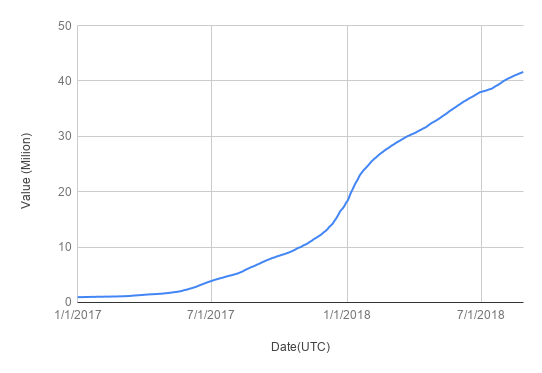
\includegraphics[width=\textwidth]{./res/img/address-growth.png}
        \caption{Unique address growth}
        \label{fig:address-chart}
    \end{subfigure}
    \begin{subfigure}[b]{0.5\textwidth}
        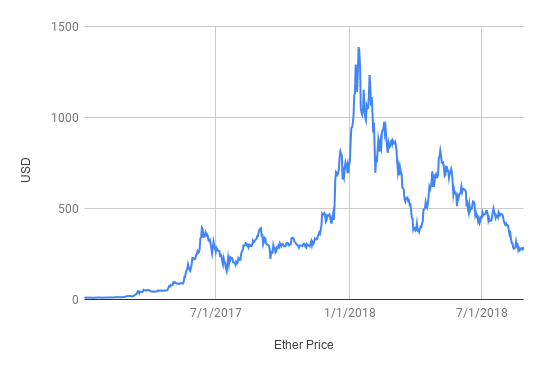
\includegraphics[width=\textwidth]{./res/img/chart_price.png}
        \caption{Ether price evolution}
        \label{fig:price-chart}
    \end{subfigure}
    \begin{subfigure}[b]{0.5\textwidth}
        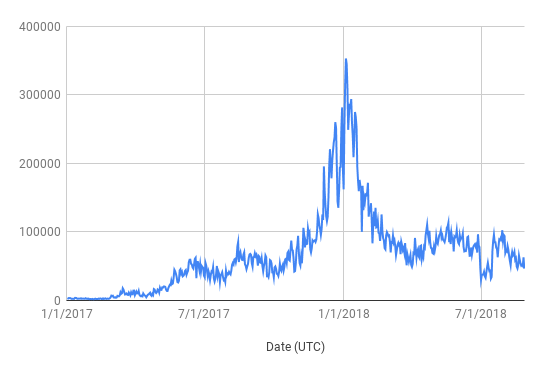
\includegraphics[width=\textwidth]{./res/img/address-growth-rate.png}
        \caption{Address growth rate}
        \label{fig:address-growth-rate-chart}
    \end{subfigure}
    \caption{Ethereum main net charts}
\end{figure*}

The size of the world state is proportional to the number of addresses, because
new addresses require an account state (\autoref{sec:world-state}).
\autoref{fig:address-chart} shows the growth in the number of address from the
beginning of $2017$. We notice that the number of unique address in the
Ethereum main net has exceeded the $40$ million units and that the growth
rate~\autoref{fig:address-growth-rate-chart} follows the price evolution of the
Ether~\autoref{fig:price-chart}, the currency of Ethereum. Indeed, around
beginning of year $2018$ the growth is no more exponential but rather linear,
because the growth rate is constant.
In addition to this, some implementation, e.g. geth, requires to store in memory
the state trees of the last $128$ 
blocks\footnote{\url{https://blog.ethereum.org/2018/02/14/geth-1-8-iceberg\%C2\%
B9/}} and when there is no place in the allocated cache it has to put some of
the old trees on storage. Therefore SSD disk are required, because otherwise it
would be too slow.

Another data-structure that should be stored is the whole blockchain. It 
consists of the block headers and also of the block bodies, i.e. the 
transactions and the uncle hashes~\cite{wood2018ethereum}. The nodes cannot
forget part of the canonical blockchain, because it can be used to rebuild 
the state. Currently, the blockchain counts more than $6$ Million blocks.

The DAG size at the genesis block is $16$ Mebibytes and it is increased of $128$
kibibytes each $30000$ blocks. So, currently, the cache is around $41$ 
Mebibytes.

The miners should store also the DAG that starts from a size of $1$ Gibibytes
and it is increased of $8$ Mebibytes, each epoch. So, currently, the DAG 
requires $2.62$ Gibibytes. So GPUs with less than $2$ Gigabytes VRAM are not
more profitable. This means that more specialized hardware are needed.



